\documentclass[12pt]{article}
\usepackage{caption}
\usepackage{graphicx}
\usepackage{hyperref}
\usepackage{amsmath}
\hypersetup{%
    pdfborder = {0 0 0}
}
\hypersetup{
    colorlinks,
    citecolor=blue,
    filecolor=blue,
    linkcolor=blue,
    urlcolor=blue
}
\renewcommand{\familydefault}{\sfdefault}
\renewcommand{\captionfont}{\small}

\author{Bernd Porr}
\title{Deep learning}

\begin{document}

\maketitle

\section{Inductive learning with Deep Learning}
We have a dataset $\vec{x}_1, \ldots, \vec{x}_N$ which should be converted
via the function
\begin{equation}
  \vec{y}=f(\vec{x}) \label{inductive}
\end{equation}
into $\vec{y}$.  The goal is to learn this function with the help of
examples $\vec{x},\vec{y}$ $\vec{x}_{N+1},\vec{y}_{N+1} \ldots$.

The following sections how learning of $f$ can be achieved.

\section{Linear neuron}

\begin{figure}[!hbt]
\begin{center}
\mbox{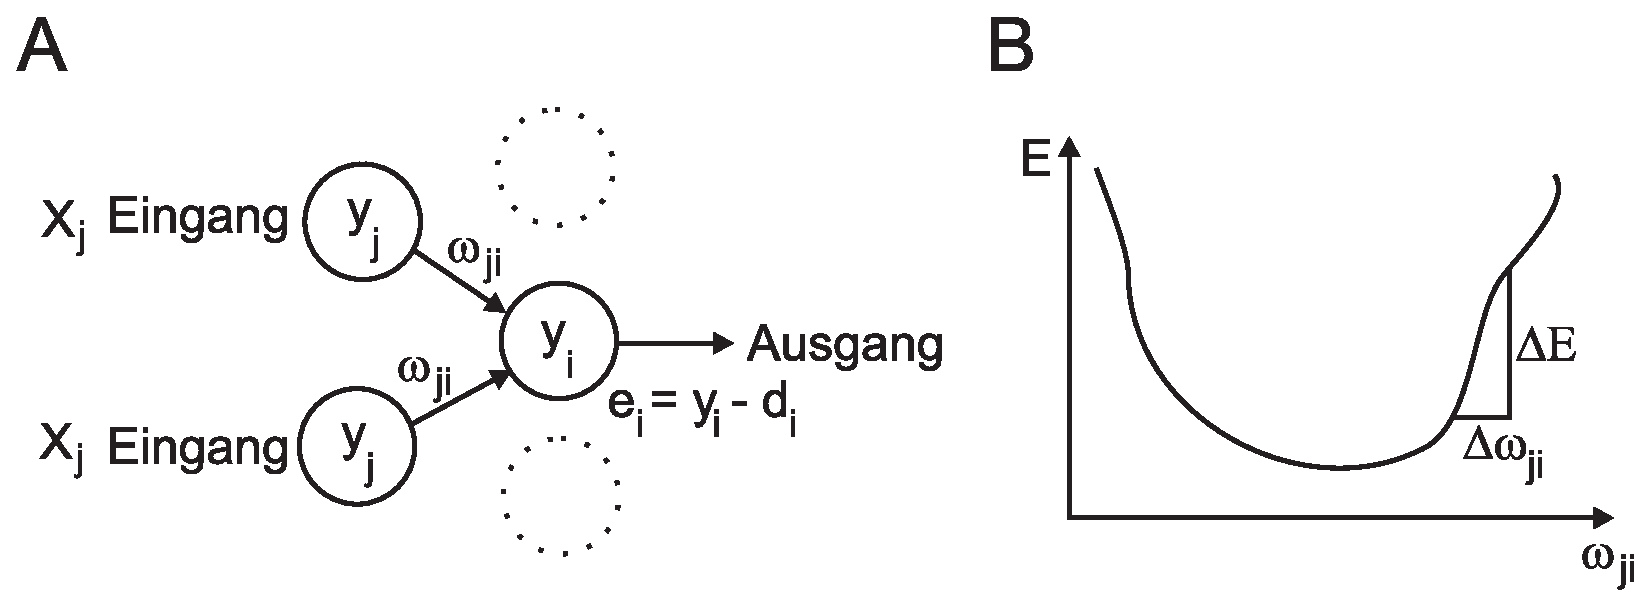
\includegraphics[width=\textwidth]{one_layer}}
\end{center}
\caption{Simple linear neuron
\label{one_layer}}
\end{figure}

Fig.~\ref{one_layer}A shows a Neuron in a single layer.
Its activation is $y(n)$ und its position $i$ in this layer which is its output.
$n$ is the current time-sample. The input activity to the neuron $x_j(n) =
y_j(n)$ is weighted by $\omega_{ji}$ and summed up to:
\begin{equation}
  y_i(n) = \sum_j y_j(n) w_{ji} \label{linear_sum}
\end{equation}
The function $f$ is here a simple linear combination of input activities where
$\omega_{ji}$ had to be learned to approximate $f$.

\section{The error signal}
The task is to learn the function $f$ which converts the input activities to output activities
(Eq.~\ref{inductive}).
This is achived by minimising the error:
\begin{equation}
  e_i(n) = y_i(n) - d_i(n) \label{output_error}
\end{equation}
where $d_i(n)$ is the desired value and $y_i(n)$ the actual output given a certain input $y_j(n)$.
The goal is to minimise the square of the error:
\begin{equation}
  E = \frac{1}{2} e^2 \label{quaderr}
\end{equation}

\section{Gradient descent}
The central trick here is to take the partial derivative in respect to the weights $\omega_{ji}$
\begin{eqnarray}
  \Delta\omega_{ji} & = & - \mu \frac{\partial E}{\partial \omega_{ji}} \label{graddes} \\
  \omega_{ji} & \leftarrow & \omega_{ji} + \Delta\omega_{ji}
\end{eqnarray}
Why does that make sense? Fig.~\ref{one_layer}B shows the relationship between error $E$ weight 
$\omega_{ji}$. In this example if the weight is slightly increased the squared error
is also increased which is not desired. Thus, it's better to decrease the weight again.
However, if increasing $\omega_{ji}$ reduces the squared error $E$ then it's a good idea
to keep that change of the weight. This approach is called \textsl{gradient descent}.

\section{Learning rule for the single layer}
We can now derive the learning rule which changes the weights $\omega_{ji}$.
We simply insert Eq.~\ref{linear_sum}, \ref{output_error} und \ref{quaderr} into Eq.~\ref{graddes}:
\begin{eqnarray}
  \Delta\omega_{ji}
   & = & - \mu \frac{1}{2} \frac{\partial ( d_i(n) - y_i(n) )^2 }{\partial \omega_{ji}} \\
   & = & - \mu \frac{1}{2} \frac{\partial \left( d_i(n) - \sum_j y_j(n) w_{ji} \right)^2 }{\partial \omega_{ji}} \\
  & = & \mu \underbrace{\left(d_i(n) - \sum_j y_j(n) w_{ji}\right)}_{-e_i(n)} \cdot y_j(n) \\
   & = & - \mu \underbrace{\frac{\partial E}{\partial y_i}}_{-e_i(n)} \underbrace{\frac{\partial y_i}{\partial \omega_{ji}}}_{y_j(n)} \label{chainrule}\\
  & = & \mu \cdot e_i(n) \cdot y_j(n) \label{learningrule}
\end{eqnarray}
where $\mu < 1$ is the learning rate or the ``step change'' so the
amount of weight change for every learning step. The learning rate is
usually very small. The learning rule Eq.\label{learningrule} is
simply a multiplication of the input activity $y_j(n)$ with the error
$e_i(n)$.


\section{Multi-layer network}
\begin{figure}[!hbt]
\begin{center}
\mbox{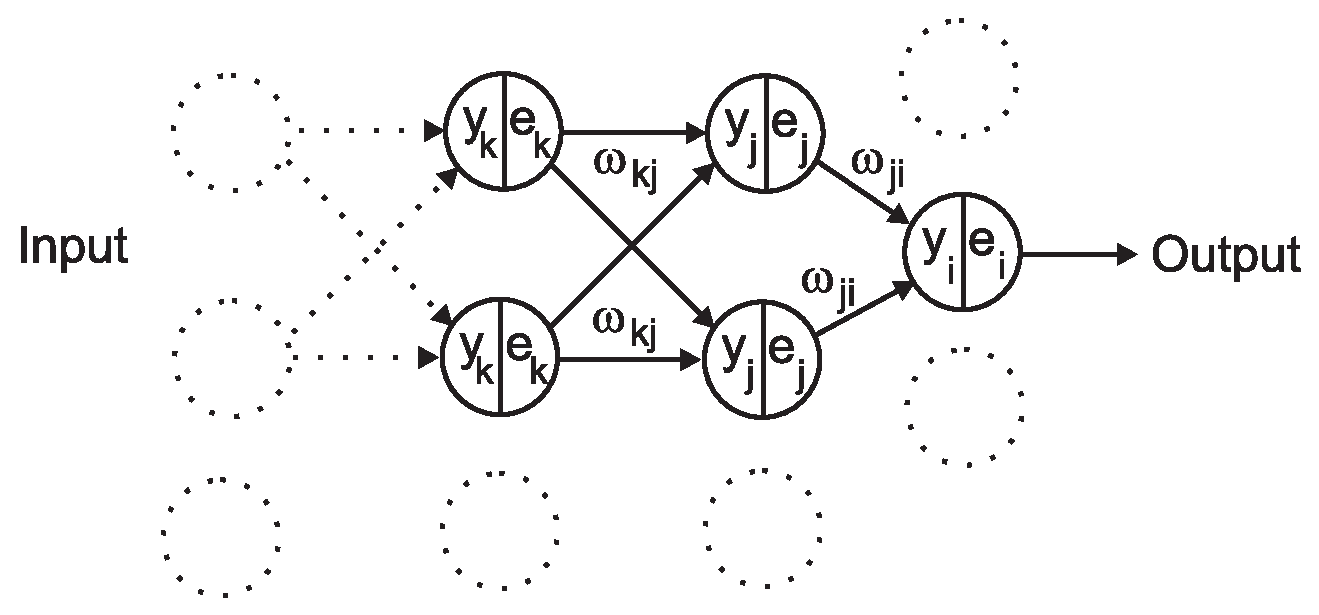
\includegraphics[width=\textwidth]{multi_layer}}
\end{center}
\caption{Mehrschichtiges Feedforward Netz
\label{multi_layer}}
\end{figure}

Abb.~\ref{multi_layer} zeigt nun ein Netzwerk mit mehreren
Schichten. Wie das Signal vom Eingang zum Ausgang durch die
verschiedenen Schichten läuft, ist einfach auszurechnen. Auch der
Fehler $e_i$ in der Ausgangsschicht kann weiterhin einfach als
Differenz zwischen $y_i$ und $d_i$ ausgerechnet werden (siehe
Gl.~\ref{output_error}). Das Problem ist, wie die \textsl{internen} Fehler
$e_j$ und $e_k$ ausgerechnet werden können.
Der interne Fehler für $\omega_{kj}$ ist erstmal genauso definiert wie der Fehler
am Ausgang (siehe Gl.~\ref{chainrule}):
\begin{equation}
  \frac{\partial E}{\partial \omega_{kj}} = \underbrace{\frac{\partial E}{\partial y_j}}_\textrm{Trick!} \frac{\partial y_j}{\partial \omega_{kj}}
  \label{gradint}
\end{equation}
aber der ist ja nicht direkt verfügbar. Der Trick ist nun den Term
$\frac{\partial E}{\partial y_j}$ mit Hilfe von der Aktivität $y_i$ am
Ausgang auszudrücken und dann einfach die beiden Terme mit
Gl.~\ref{linear_sum} und Gl.~\ref{chainrule} zu identifizieren:
\begin{equation}
  \frac{\partial E}{\partial y_j} = \sum_i \underbrace{\frac{\partial E}{\partial y_i}}_{-e_i} \cdot \underbrace{\frac{\partial y_i}{\partial y_j}}_{\omega_{ji}} \label{dltrick}
\end{equation}
Gl.~\ref{dltrick} wieder in Gl.~\ref{gradint} substituiert gibt dann:
\begin{equation}
  \frac{\partial E}{\partial \omega_{kj}} = - \left( \sum_i e_i \omega_{ji} \right) \frac{\partial y_j}{\partial \omega_{kj}}
  \label{gradintback}
\end{equation}
mit
\begin{equation}
y_j = \sum_k y_k(n) w_{kj}
\end{equation}
führt das zu:
\begin{eqnarray}
  \frac{\partial E}{\partial \omega_{kj}} & = & - \left( \sum_i e_i \omega_{ji} \right) \underbrace{\frac{\partial \left(\sum_k y_k(n) w_{kj}\right)}{\partial \omega_{kj}}}_{y_k} \\
                                         & = & - \left( \sum_i e_i \omega_{ji} \right) y_k
\end{eqnarray}
Die Änderung des internen Gewichtes $\omega_{kj}$ folgt dann folgender Gleichung:
\begin{equation}
\Delta\omega_{kj} = \mu \cdot y_k \cdot \underbrace{\sum_i e_i \omega_{ji}}_{e_j}
\end{equation}
Wobei nun $e_j$ der interne Error ist und damit ist es möglich, alle internen Fehler rückwärts vom Ausgang zum Eingang zu berechnen.

\begin{figure}[!hbt]
\begin{center}
\mbox{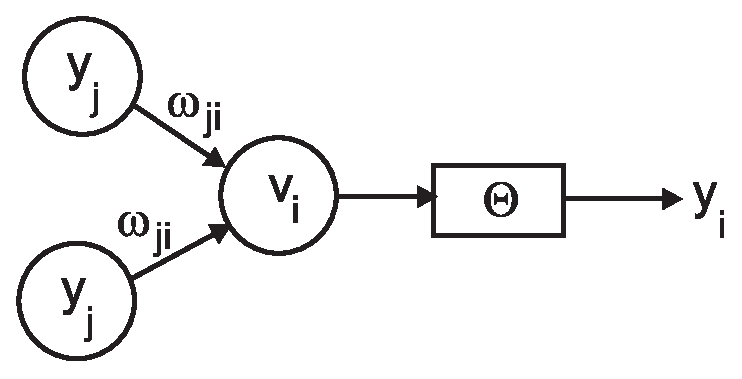
\includegraphics[width=0.5\textwidth]{nonlin}}
\end{center}
\caption{Neuron mit nichtlinearer Characteristik
\label{nonlin}}
\end{figure}

\section{Nicht-lineare Netzwerke}
Nur wenn Netzwerke nicht-linear sind, machen tiefere Schichten einen
Sinn, da jedes lineare Netzwerk immer auf eine Schicht reduziert
werden kann.  Erst die Nichtlinearität rechtfertigt tiefe (``deep'')
mehrschichtige Netzwerke.  Abb.~\ref{nonlin} zeigt ein Neuron von
solch einem mehrschichtigen Netzwerk, wo die lineare Summe dann durch
eine Nichtlinearität geschickt wird:
\begin{equation}
  y_i(n) = \Theta\left(\underbrace{\sum_j y_j(n) w_{ji}}_{v_i} \right) \label{nonlinear_sum}
\end{equation}
Was aendert sich in diesem Fall an den Lernregeln? Sehr wenig. Wenn man sich Gl.~\ref{chainrule} ansieht, merkt man, dass einfach
ein weiterer Term durch die Kettenregel hinzukommt:
 \begin{equation}
 \frac{\partial E}{\partial \omega_{ji}}  = \frac{\partial E}{\partial y_i} \underbrace{\frac{\partial y_i}{\partial v_i}}_{\Theta^\prime} \frac{\partial v_i}{\partial \omega_{ji}}
 \end{equation}
 wo $\Theta^\prime$ einfach die Ableitung der nicht-linearen Aktivierungsfunktion $\Theta$ ist. Das heißt, dass der Fehler für die
 Ausgangsschicht jetzt folgendermaßen ausgerechnet wird:
\begin{equation}
  \Delta\omega_{ji} = \mu \cdot \Theta^\prime(y_i) \cdot y_j \cdot e_i 
\end{equation}
und der interne Fehler so:
\begin{equation}
\Delta\omega_{kj} = \mu \cdot \Theta^\prime(y_j) \cdot y_k \cdot \underbrace{\sum_i e_i \omega_{ji}}_{e_j} 
\end{equation}

Strikt muss die nicht-lineare Funktion $\Theta$ differenzierbar
sein. Es hat sich aber herausgestellt, dass der Einweggleichrichter
(Rectifiying Linear Unit = ReLU)
\begin{equation}
  \Theta(v) =
  \begin{cases}
    0, & \text{falls}\ v < 0 \\
    v, & \text{ansonsten}
  \end{cases}
\end{equation}
für viele Klassifizierungen am besten
ist. Dessen Ableitung hat keine eindeutige Lösung am Ursprung so dass man sich dort
entscheiden muss, ob sie eins oder Null ist. Andere populäre nicht-lineare
Funktionen sind $\Theta(v)=\tanh(v)$ oder die sigmoide Funktion: $\Theta(v)=\frac{1}{1+e^{-v}}$.




\end{document}
